\def\theTopic{Inference on Proportions }
\def\dayNum{8}

\begin{center}
{\bf {\large MIT -- the Male Idiot Theory}}
\end{center}

\begin{enumerate}
   \item  What is the parameter of interest?
\begin{students}
    \vspace{1cm}    
\end{students}
\begin{key} 
  {\it $p$ = the proportion of all idiots who are male.}
\end{key}
  \item \label{MIT.phat} What statistic do we obtain from the sample?
    Give proper notation, the statistic's value, and explain it in words.
\begin{students}
    \vspace*{2cm}    \\
\end{students}
\begin{key} 
   { $\widehat{p} = \frac{282}{318} = 0.887$ \it is the
    proportion of the sample which is male.}
\end{key}
\item Looking at the research question, ``Is the group of idiots in the world
  more than half male?'',   we set
  up the null hypothesis to assume ``just half'' and the alternative to be
  ``more than half'' male.
    \begin{enumerate}
    \item State null and alternative hypotheses in symbols and
      words.\\
      $H_0:$ 
\begin{students}
    \vspace{1.5cm}    \\
\end{students}
\begin{key} 
{\it $p = .5$.  Half of all idiots are male.}
\end{key}
$H_a:$
\begin{students}
    \vspace{1cm}    \\
\end{students}
\begin{key} 
{\it $p > .5$.  More than half of all idiots are male.}
\end{key}
    \item How would you mark cards and randomly draw from them (or use
      another random method) to
      obtain one simulated proportion drawn from the distribution when
      $H_0$ is true?
\begin{students}
    \vspace{3cm}    
\end{students}
\begin{key} 
  {\it Take an even number of cards (could be 318, but a
    smaller number will also work). Mark half of them male, half
    female. Shuffle and draw one. Record the gender. Return the card
    to the deck, repeat 317 more times and divide the total number of
    males by 318 to get one sample proportion.}
\end{key}
    \item Input the data under \fbox{One Categ} in 
      \url{https://jimrc.shinyapps.io/Sp-IntRoStats}
      and then select the  \fbox{Test} page.  Do we need to change the
      ``Null value'' for $p$?\\ \ \\
      Click \fbox{1000} several times to get a distribution of sample
      proportions under $H_0$. 
      Sketch the picture you get here.
\begin{students}
    \vspace{5cm}    
\end{students}
\begin{key}
\ \  \\ 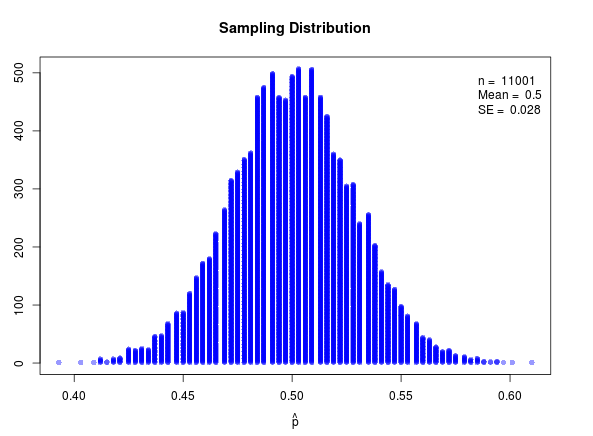
\includegraphics[width=.3\linewidth]{../plots/MIT-null.png}
\end{key}
  \item How unusual is the sample statistic from \ref{MIT.phat}
    relative to the distribution you created?  Explain in words where
    it falls relative to the plotted points.
\begin{students}
    \vspace{3cm}    
\end{students}

\begin{key}
{\it It's much bigger than any of the points I generated. The largest
  one I got was 0.585 or 186 males out of 318.}
\end{key} 
\item  How strong is the evidence against the null hypothesis?  What
  do you think about the idea that idiots are half male?
\begin{students}
    \vspace{2cm}    
\end{students}

\begin{key}
  {\it Extremely strong evidence, the p-value is less than 1 in
    1000. The null hypothesis of only half males is not 
    supported by these data. I conclude that there are more male idiots
  than female idiots.  } 
\end{key}


\end{enumerate}

\item Instead of considering a test of the true population proportion, we
  will switch gears and now estimate it.
  \begin{enumerate}
    \item What is our ``point'' estimate of the
      true proportion of idiots who are male (the sample statistic)?
\begin{students}
    \vspace{.4cm}    
\end{students}

\begin{key}
$\widehat{p} = 0.887$
\end{key}
    \item In order to generate simulated data,
      \begin{enumerate}
        \item How many individual ``idiots'' do we generate for one
          resample?
\begin{students}
    \vspace{.8cm}    
\end{students}

\begin{key} 
$318$
\end{key}
       \item Explain how you would mark 318 cards and use them to
         simulate the gender of one individual, and then another.
\begin{students}
    \vspace{2.5cm}    
\end{students}

\begin{key} 
  {\it Mark 26 ``Female'' and 282 ``Male''.  Shuffle them and draw one
  at random.  Replace the card, remix, and draw again for the second
  person.} 
\end{key}
       \item What probability of being male is used?
\begin{students}
    \vspace{.5cm}    
\end{students}

\begin{key} 
  {$0.887$}
\end{key}
       \item After resampling 318 individuals, what number do you compute?
\begin{students}
    \vspace{1.2cm}    
\end{students}

\begin{key} 
  {\it  The proportion of the 318 new draws which are male.}
\end{key}
     \end{enumerate}
     \item Use the  web applet to create  1000 or more
       resamples from the original data. 
       \begin{enumerate}
         \item Where is this distribution centered?
\begin{students}
    \vspace{.7cm}    
\end{students}

\begin{key} 
  {\it  0.887}
\end{key}
         \item What is the spread of the distribution of resampled proportions?
\begin{students}
    \vspace{.7cm}    
\end{students}

\begin{key} 
  {\it SE =  0.018}
\end{key}
         \end{enumerate}
     \item Find a 95\% confidence interval for the true proportion of
       idiots who are male.
\begin{students}
    \vspace{1.2cm}    
\end{students}

\begin{key} 
  $  (0.852, 0.925)$
\end{key}
     \item \label{longRun}Explain what the word ``confidence'' means for this
       confidence interval.
\begin{students}
    \vspace{3cm}    
\end{students}

\begin{key} 
  {\it Our confidence is in the process, not in just one interval. If
    we repeat the process (gather a new random sample) over and over,
    95\% of the intervals we create will include the true parameter of
  interest.}
\end{key}

  \end{enumerate}
\item Interpret this confidence interval.
\begin{students}
    \vspace{2cm}    
\end{students}

\begin{key} 
  {\it We are 95\% confident that the true percentage of idiots who
    are male is between 85.2\% and 92.5\%.}
\end{key}


\item Compare results from the hypothesis test and the interval
  estimate.  If the null hypothesis is true, what value should be
  included in the 95\% CI?  Explain. Do the two methods agree to some
  extent? 
\begin{students}
    \vspace{2.5cm}    
\end{students}

\begin{key} 
  {\it  If $H_0$ is true, then the interval should contain 0.50.  It
    does not, so the two inferences agree that one--half is not
    consistent with the data.} 
\end{key}
\end{enumerate}


\begin{center}
  {\bf Take Home Message:} \vspace{-.3in}
\end{center}
\begin{itemize}
  \item You just did two inferences on the same parameter.  First, we
    tested the null hypothesis that half the world's idiots are
    male.\\
      You should have reported very strong evidence against that null
      hypothesis (less than 1/1000). We can feel quite confident that
      the true proportion 
      of males in this exclusive group is more than one half.

  \item Secondly, we computed a 95\% confidence interval for the true
    proportion of idiots who are male and you interpreted the
    interval.  In \ref{longRun} you should have explained the
    long--run coverage property of the method.
  \item   There is a correspondence
    between testing and estimating.  The values inside the interval
    you found are consistent with the data, or {\bf plausible}.  Because
    0.50 is not in the interval, it is not a plausible value for this
    parameter. 
 \item 
  Questions? Make your own summary of the  lesson. 
\end{itemize}

%% Not yet using `reject the null' terminology.



\noindent
{\bf Assignment}
\begin{itemize}
\item D2Quiz 4 is due Feb 8.
\item Review for the exam.
\item Read pages 69--71 for Friday or Tuesday after the exam.
\end{itemize}
